\section{Feature-Sensitive Coverages}\label{sec:fscov}

This section first formulates the general definition of graph coverages for a
given directed graph and explains representative coverage metrics as examples.
%
Then, we introduce a \textit{feature-sensitive (FS) coverage} as a general
extension of graph coverages to fully discriminate semantics between different
language features.
%
Finally, we define a \textit{feature call path-sensitive (FCPS) coverage} as a
variant of FS coverage to distinguish different parts in the semantics of the
same language features.


%----------------------------------------%
%----------------------------------------%


\subsection{Notations}\label{sec:notation}
%
First, we define notations used in the definition of graph coverages.
%
A \textit{directed graph} $\graph = (\nodeset, \inodeset,
\fnodeset, \edgeset)$ consists of:
\begin{itemize}
  \item a set of \textit{nodes} $\nodeset$
  \item a set of \textit{initial nodes} $\inodeset \subseteq \nodeset$
  \item a set of \textit{final nodes} $\fnodeset \subseteq \nodeset$
  \item a set of \textit{edges} $\edgeset \subseteq \nodeset \times \nodeset
    \times (\annotset \uplus \{ \bot \})$ with a set of \textit{annotations}
    $\annotset$
\end{itemize}
%
The notation $\node \edge{\annot} \node'$ denotes an edge from a node $\node$ to
a node $\node'$ with an annotation $\annot \in \annotset$.
%
If an edge has an empty annotation $\bot$, we omit the annotation: $\node
\edge{} \node'$.
%
In a given directed graph $\graph$, a \textit{path} $\pat \in \patset{\graph}$
is a sequence of one or more nodes, where each pair of adjacent nodes is an
edge:
\begin{equation}\label{euq:path-def}
  \patset{\graph} = \{
    \node_0 \edge{\annot_0} \cdots \edge{\annot_{m-1}} \node_m \mid
    \forall i < m. \; \node_i \edge{\annot_i} \node_{i+1} \in \edgeset \wedge
    \node_m \in \nodeset
  \}
\end{equation}
%
The length of a path is defined as $\norm{\node_0 \edge{\annot_0} \cdots
\edge{\annot_{m-1}} \node_m} = m$.
%
A path $\pat$ is a \textit{subpath} ($\subpath$) of a path $\pat'$ when $\pat$
is a subsequence of $\pat'$.
%
We use the notation $\prefix$ for a prefix relation, and $\getfirst(\pat)$ and
$\getlast(\pat)$ denote the first and last nodes of the path $\pat$,
respectively.
%
A path $\pat$ is \textit{full} when it starts at an initial node and ends at a
final node: $\getfirst(\pat) \in \inodeset \wedge \getlast(\pat) \in \fnodeset$.
%
Then, $\patmap{\graph} : \testset \rightarrow \patset{\graph}$ is a mapping from
a \textit{test} $\test \in \testset$ to a full path in the graph $\graph$, and
we call $\patmap{\graph}(\test)$ as the \textit{execution path} of $\test$.

%----------------------------------------%

\paragraph{\textbf{Example}}
%
Consider a control-flow graph (CFG) $\graph$ depicted in
Figure~\ref{fig:spec-cfg} and the following JavaScript programs as a test set $T
\subseteq \testset$:
\begin{equation}\label{equ:testset}
  T = \left\{
    \begin{array}{rcl}
      \cdots\\
      \addtest &=& \text{(a JavaScript program \jscode{2n + 1;})}\\
      \subtest &=& \text{(a JavaScript program \jscode{2n - 1;})}\\
      \cdots\\
    \end{array}
  \right.
\end{equation}
%
Then, $\patmap{\graph}(\addtest)$ is the execution path of $\addtest$:
\[
  \small
  \!\begin{array}{l}
    \cdots
    \call \overset{\text{{\bf Evaluation} of \esnt{AdditiveExpression}
      \esconst{+} \esnt{MultiplicativeExpression}}}{\rcolorbox{gray3}{\(
    1
    \call
    \overset{\textbf{EvaluateStringOrNumericBinaryExpression}}{\rcolorbox{gray2}{\(
    7 \edge{} \cdots \edge{} 8
    \call \overset{\textbf{ApplyStringOrNumericBinaryOperator}}{\colorbox{gray1}{\(
    11 \edge{} \cdots \edge{} 12
    \call \overset{\textbf{ToNumeric}}{\colorbox{white}{\(
    19 \edge{} \cdots \edge{} 20 \tedge \colorbox{lightred}{21} \edge{} 22
    \)}}
    \ret 13 \fedge 14
    \)}}
    \)}}
    \)}}

    \vspace*{1em}\\

    \lcolorbox{gray3}{\(
    \lcolorbox{gray2}{\(
    \colorbox{gray1}{\(
    \call \overset{\textbf{ToNumeric}}{\colorbox{white}{\(
    19 \edge{} \cdots \edge{} 20 \fedge \cdots \edge{} 22
    \)}}
    \ret 15 \fedge 16 \tedge \colorbox{lightred}{17} \edge{} 18
    \)}
    \ret 9 \tedge 10
    \)}
    \ret 2 \tedge 3
    \)}
    \ret \cdots\\
  \end{array}
\]
And, $\patmap{\graph}(\subtest)$ is equal to $\patmap{\graph}(\addtest)$ except
for nodes 4, 5, and 6 in the $\textbf{Evaluation}$ SDO for subtraction rather
than 1, 2 and 3 in the $\textbf{Evaluation}$ SDO for addition.
%
The following path $\pat$ is a subpath of both $\patmap{\graph}(\addtest)$ and
$\patmap{\graph}(\subtest)$:
\begin{equation}\label{equ:subpath}
  \pat = 22 \ret 15 \fedge 16 \tedge \colorbox{lightred}{17}
\end{equation}
whose length is $\norm{\pat} = 3$.


%----------------------------------------%
%----------------------------------------%


\subsection{Graph Coverages}\label{sec:cov}

We formulate graph coverages by referring to their well-known
definitions~\cite{testing}.
%
For a given directed graph, we specify \textit{graph coverage} criteria by 1) a
set of \textit{test requirements} and 2) a \textit{cover relation} between paths
and test requirements:

%----------------------------------------%

\begin{definition}[Graph Coverage]\label{def:graph-cov}
  A \textit{graph coverage} criterion $\cov{\graph} = (\trset{\graph}, \cover)$
  for a given directed graph $\graph$ is defined with:
  \begin{itemize}
    \item a set of \textit{test requirements (TRs)} $\trset{\graph}$
    \item a \textit{cover relation} $\cover \subseteq \patset{\graph} \times
      \trset{\graph}$ between paths and TRs
  \end{itemize}
\end{definition}

%----------------------------------------%

In a specific graph coverage criterion $\cov{\graph}$, we say that a path $\pat$
\textit{covers} a TR $\tr \in \trset{\graph}$ when $\pat \cover
\tr$.
%
We also say that a test $\test \in \testset$ covers the TR $\tr$ if there exists
a prefix path $\pat$ of its execution path covers the TR:
%
\begin{equation}\label{equ:test-cover}
  \test \cover \tr
  \iff
  \exists \pat \in \patset{\graph}. \tst
  \pat \prefix \patmap{\graph}(\test) \wedge
  \pat \cover \tr
\end{equation}
%
A test set $T \subseteq \testset$ \textit{satisfies} ($\sat$) the criterion
$\cov{\graph}$ when it covers all valid TRs:
\begin{equation}\label{equ:sat}
  T \sat \cov{\graph}
  \iff
  \forall \tr \in \trset{\graph}. \;
  \tr \; \text{is valid} \; \Rightarrow
  \exists \test \in T. \tst \test \cover \tr
\end{equation}
where a TR $\tr$ is \textit{valid} if there exists a possible test $\test \in
\testset$ that covers $\tr$.
%
If $T \sat \cov{\graph} \Rightarrow T \sat \cov{\graph}'$ for any test set $T$,
we say that $\cov{\graph}$ \textit{subsumes} $\cov{\graph}'$ and use the
notation: $\cov{\graph} \subs \cov{\graph}'$.
%
The subsumption relation between graph coverage criteria is a partial order.

%----------------------------------------%

\begin{definition}[Node Coverage]\label{def:node-cov} In a \textit{node
  coverage} criterion $\nodecov{\graph}$,
  \begin{itemize}
    \item the set of \textbf{TRs} $\trset{\graph}$ is a set of nodes:
      \[
        \trset{\graph} = \nodeset
      \]
    \item a path $\pat$ \textbf{covers} a node $\node$ when it ends with the
      node $\node$:
      \[
        \pat \cover \node \iff \getlast(\pat) = \node
      \]
  \end{itemize}
\end{definition}

%----------------------------------------%

The node coverage is the most common graph coverage defined with nodes as test
requirements, and we could generalize it into \textit{$k$-limiting path
coverage} criteria using paths instead of nodes:

%----------------------------------------%

\begin{definition}[$k$-Limiting Path Coverage]\label{def:k-path-cov}
  In a \textit{$k$-limiting path coverage} criterion $\kpathcov{k}{\graph}$,
  \begin{itemize}
    \item the set of \textbf{TRs} $\trset{\graph}$ is a set of
      paths whose lengths are bounded by $k$:
      \[
        \trset{\graph} = \{ \pat \in \patset{\graph} \mid \norm{\pat} \leq k \}
      \]
    \item a path $\pat$ \textbf{covers} a path $\pat'$ when their last nodes are
      equal and the path $\pat'$ is a subpath of $\pat$:
      \[
        \pat \cover \pat'
        \iff
        \getlast(\pat) = \getlast(\pat') \wedge \pat' \subpath \pat
      \]
  \end{itemize}
\end{definition}

%----------------------------------------%

Now, a node coverage could be redefined as $0$-limiting path coverage
($\kpathcov{0}{\graph} = \nodecov{\graph}$), and other graph coverages are
defined with $k$-limiting path coverages as well:
\begin{itemize}
  \item An \textit{edge coverage} criterion is $\kpathcov{1}{\graph}$
  \item An \textit{edge-pair coverage} criterion is $\kpathcov{2}{\graph}$
  \item A \textit{complete path coverage} criterion is
    $\kpathcov{\infty}{\graph}$
\end{itemize}
%
Note that $k$-limiting path coverage criteria utilize the inequality for path
lengths $\norm{\pat} \leq k$ rather than equality $\norm{\pat} = k$.
%
Thus, if $i \leq j$, the set of TRs in $\kpathcov{i}{\graph}$ is always a subset
of that in $\kpathcov{j}{\graph}$, and $\kpathcov{j}{\graph}$ subsumes
$\kpathcov{i}{\graph}$.
%
A \textit{branch coverage} criterion is a variant of an edge coverage that
treats only out-edges of conditional branches as TRs.
%
It is possible to merge multiple coverage criteria by defining unions of TRs and
cover relations as the TR and cover relation of the merged coverage criterion.
%
For example, a \textit{node-or-branch coverage} criterion is a merged
criterion of node and branch coverage criteria.

%----------------------------------------%

A complete path coverage might have infinite TRs because of recursions and loop
structures.
%
To resolve this problem, \citet{testing} have presented a \textit{simple path
coverage} that deals with only simple paths as TRs.
%
A path $\node_0 \edge{\annot_0} \cdots \edge{\annot_{m-1}} \node_m$ is
\textit{simple} if no duplicated nodes in the path, with the exception that the
first and last nodes may be identical: $\forall i, j. \; \node_i = \node_j
\Rightarrow (i = j \vee \{ i, j \} = \{ 0, m \})$.
%
In addition, they extend it to a \textit{prime path coverage} to reduce the
number of TRs by filtering out meaningless simple paths.
%
It deals with only prime paths as TRs, where a \textit{prime path}
is a maximal length simple path in the graph.
%
However, such advanced structural coverage criteria still need a tremendous
number of TRs for the entire control-flow graphs.
%
Hence, they are commonly used only for unit testing~\cite{unit-test} in practice
with intra-procedural control-flow graphs.

%----------------------------------------%

\paragraph{\textbf{Example}}
%
Consider again a CFG $\graph$ depicted in Figure~\ref{fig:spec-cfg} and the test
set $T$ in (\ref{equ:testset}), including $\addtest$ and $\subtest$.
%
If we measure the $3$-limiting path coverage $\kpathcov{3}{\graph}$ for the test
set $T$, both a node 17 and the path $\pat$ in (\ref{equ:subpath}) are test
requirements $\trset{\graph}$.
%
First, the prefix path, whose last node is 17, of $\patmap{\graph}(\addtest)$
covers both TRs: node 17 and $\pat$.
%
Thus, the test $\addtest$ for addition covers both of them.
%
Similarly, the test $\subtest$ for subtraction covers both of them for the same
reason.
%
Unfortunately, it causes that either $\addtest$ or $\subtest$ might be removed
in the minimal test set because they cover the same TRs, node 17 and the path
$\pat$.


%----------------------------------------%
%----------------------------------------%


\subsection{Feature-Sensitive (FS) Coverages}\label{sec:fs-cov}

To alleviate the problem explained in Section~\ref{sec:diff-feat}, we introduce
a novel \textit{feature-sensitive (FS) coverage} as a general extension of any
graph coverages.
%
It depends on the following two components:
%
\begin{itemize}
  \item a set of \textit{language features} $\featset$
  \item a \textit{feature mapping} $\featmap: \nodeset \rightarrow \featset
    \uplus \{ \bot \}$, a partial mapping from nodes to language features.
\end{itemize}
%
where $\featmap(\node) = \bot$ means that there is no language feature for the
node $\node$.

%----------------------------------------%

We first define the \textit{call-site stack} $\css{\pat} \in \nodeset^*$ of a
path $\pat$ as a sequence of nodes constructed by:
\begin{equation}\label{equ:css}
  \css{\pat} = \left\{
    \begin{array}{ll}
      \epsilon &
      \tif \pat = \node\\

      {[\node_1, \cdots, \node_m, \getlast(\pat')]} &
      \tif \pat = \pat' \call \node \wedge
      \css{\pat'} = [\node_1, \cdots, \node_m]\\

      {[\node_1, \cdots, \node_{m-1}]} &
      \tif \pat = \pat' \ret \node \wedge
      \css{\pat'} = [\node_1, \cdots, \node_m]\\

      \css{\pat'} &
      \tif \pat = \pat' \edge{\annot} \node

    \end{array}
  \right.
\end{equation}
In other words, $\css{\pat}$ keeps only call-sites not matched with return-sites
in the path $\pat$.  A \textit{call-site} is a node having a call edge ($\call$)
as its out-edge, and a \textit{return-site} is a node having a return edge
($\ret$) as its in-edge.
%
Then, we define the \textit{feature extractor} $\extfeat: \css{\patset{\graph}}
\rightarrow \featset \uplus \{ \bot \}$ as a partial mapping from call-site
stacks to enclosing language features $\featset$:
\begin{equation}\label{equ:extfeat}
  \extfeat([\node_1, \cdots, \node_m]) = \left\{
    \begin{array}{ll}
      \feat & \tif
      \exists i. \tst \featmap(\node_i) = \feat \wedge
      \forall j > i. \; \featmap(\node_j) = \bot
      \\

      \bot & \telse
    \end{array}
  \right.
\end{equation}
%
Similarly, $\extfeat(\css{\pat}) = \bot$ means that there is no language feature
for the path $\pat$.

%----------------------------------------%

\begin{definition}[Feature-Sensitive (FS) Coverage]\label{def:fs-cov}
  For a given graph coverage $\cov{\graph} = (\trset{\graph}, \cover)$, the
  \textit{feature-sensitive (FS) coverage} $\fcov{\graph} = (\ftrset{\graph},
  \cover)$ is defined as follows:
  \begin{itemize}
    \item the set of \textbf{feature-sensitive test requirements (FS-TRs)}
      $\ftrset{\graph}$ is a set of original TRs optionally tagged with language
      features:
      \[
        \ftrset{\graph} = \trset{\graph} \times (\featset \uplus \{ \bot \})
      \]
    \item a path $\pat$ \textbf{covers} a FS-TR $(\tr, \feat)$ when $\pat$
      covers the original TR $\tr$ and $\feat$ is the enclosing language feature
      of $\pat$:
      \[
        \pat \cover (\tr, \feat) \iff \pat \cover \tr \wedge
        \extfeat(\css{\pat}) = \feat
      \]
  \end{itemize}
\end{definition}

%----------------------------------------%

\paragraph{\textbf{Example}}
%
For the CFG $\graph$ depicted in Figure~\ref{fig:spec-cfg}, we could define the
feature mapping $\featmap$ as follows:
\begin{equation}\label{equ:featmap}
  \featmap(\node) = \left\{
    \begin{array}{ll}
      \addfeat & \tif \node \in \{ 1, 2, 3\} \\
      \subfeat & \tif \node \in \{ 4, 5, 6\} \\
      \numfeat & \tif \node \in \{ 23, 24, 25, 26 \} \\
      \bot & \telse
    \end{array}
  \right.
\end{equation}
%
Consider two tests $\addtest$ and $\subtest$ in the test set $T$
(\ref{equ:testset}), and two prefix paths $\addpat$ and $\subpat$, whose last
nodes are 17, of their execution paths:
%
\begin{equation}\label{equ:prepath}
  \begin{array}{rclcl}
    \addpat &=& \cdots \tedge 17 &\tst&
    \addpat \prefix \patmap{\graph}(\addtest)\\

    \subpat &=& \cdots \tedge 17 &\tst&
    \subpat \prefix \patmap{\graph}(\subtest)\\
  \end{array}
\end{equation}
%
First, the call-site stack of $\addpat$ is $\css{\addpat} = [\cdots, 1, 8]$
because other call-sites 12 and 14 are removed by matched return-sites 13 and
15, respectively.
%
Since there is no feature mapping for the call-site 8, the enclosing language
feature of $\addpat$ is $\extfeat(\css{\addpat}) = \featmap(1) = \addfeat$.
%
Hence, if we use a FS node coverage $\fnodecov{\graph}$, the path $\addpat$
covers a FS-TS $(17, \addfeat)$, and the test $\addtest$ for addition covers it
as well.
%
In a similar way, we know that the enclosing language feature of $\subpat$
is $\extfeat(\css{\subpat}) = \featmap(4) = \subfeat$.
%
It means that $\subtest$ covers a new FS-TS $(17, \subfeat)$ instead of $(17,
\addfeat)$ and remains in the minimal test set.

%----------------------------------------%

In addition, we extend the feature extractor $\extfeat$ to apply $k$-limiting
approach to FS coverages. The extended feature extractor $\extfeats{k}:
\css{\patset{\graph}} \rightarrow \featset^{\leq k}$ collects at most $k$
enclosing language features:
%
\begin{equation}\label{equ:extfeats}
  \extfeats{k}([\node_1, \cdots, \node_m]) = \left\{
    \begin{array}{ll}
      \epsilon & \tif k = 0 \vee m = 0\\

      \extfeats{k-1}([\node_1, \cdots, \node_{m-1}]) + \feat & \tif
      \featmap(\node_m) = \feat\\

      \extfeats{k}([\node_1, \cdots, \node_{m-1}]) & \telse\\
    \end{array}
  \right.
\end{equation}

%----------------------------------------%

\begin{definition}[$k$-Limiting Feature-Sensitive ($k$-FS)
  Coverage]\label{def:k-fs-cov}
  For a given graph coverage $\cov{\graph} = (\trset{\graph}, \cover)$, the
  \textit{$k$-limiting feature-sensitive ($k$-FS) coverage} $\kfcov{k}{\graph} =
  (\kftrset{k}{\graph}, \cover)$ is defined as follows:
  \begin{itemize}
    \item the set of \textbf{$k$-feature-sensitive test requirements
      ($k$-FS-TRs)} $\kftrset{k}{\graph}$ is a set of original TRs tagged with
      at most $k$ language features:
      \[
        \kftrset{k}{\graph} = \trset{\graph} \times \featset^{\leq k}
      \]
    \item a path $\pat$ \textbf{covers} a $k$-FS-TR $(\tr, \feats)$ when $\pat$
      covers the original TR $\tr$ and $\feats$ is the $k$-most enclosing
      language features of $\pat$:
      \[
        \pat \cover (\tr, \feats) \iff \pat \cover \tr \wedge
        \extfeats{k}(\css{\pat}) = \feats
      \]
  \end{itemize}
\end{definition}

%----------------------------------------%

\paragraph{\textbf{Example}}
%
Now, consider the following JavaScript program as a test $\test$ with the graph
in Figure~\ref{fig:spec-cfg}:
\[
  \begin{array}{rcl}
    \test \in \testset &=&
    \text{(a JavaScript program \jscode{[] - (2n + 1);})}\\
  \end{array}
\]
Then, it throws a \textbf{TypeError} exception in node 17 during the execution
of the expression \jscode{2n + 1}.
%
Consider the prefix path $\pat$, whose last node is 17, of the execution path of
$\test$.
%
Then, $\extfeats{2}(\pat) = [\subfeat, \addfeat]$ because the most enclosing
language feature is $\addfeat$, and the next enclosing one is $\subfeat$ for the
path $\pat$.
%
If we use $2$-FC node coverage $\kfnodecov{2}{\graph}$, the set of $2$-FS-TRs is
$\kftrset{2}{\graph} = (\nodeset, \featset^{\leq 2})$, and the test $\test$
covers a $2$-FS-TR $(17, [\subfeat, \addfeat])$.

%----------------------------------------%

% XXX not a good example of k-FS for k >= 2. please find another
The $k$-FS coverage divides TRs using each combination of different language
features.
%
Especially, the $k$-FS coverage with $k \geq 2$ is helpful to cover edge cases in
JavaScript engines and transpilers because they are heavily optimized and handle
even same language features differently depending on which language features are
used together.
%
For example, a \jscode{let} declaration just declares a block-scoped local
variable.
%
However, JavaScript engines and transpilers often have a different execution path
to handle it when it is declared in a \jscode{for-in/of} statement rather than a
simple block.
%
Indeed, the GraalJS~\cite{graaljs} engine and the Babel~\cite{babel} transpiler
contain conformance and crashing bugs only reproducible with a combination of
\jscode{let} declaration and \jscode{for-in/of} statement.\footnote{
  See \url{https://github.com/oracle/graaljs/issues/656} and
  \url{https://github.com/babel/babel/issues/15100}
}

%----------------------------------------%
%----------------------------------------%

\subsection{Feature Call Path-Sensitive (FCPS) Coverages}\label{sec:fcps-cov}

As explained in Section~\ref{sec:same-feat}, a more fine-grained set of test
requirements is necessary to distinguish different parts of the semantics even
in the same language features.
%
To resolve this problem, we define a \textit{feature call path-sensitive (FCPS)
coverage} as a variant of FS coverage.
%
The main idea of FCPS coverage is to distinguish TRs using paths from the most
enclosing language features.
%
However, if we keep paths as it is, the number of TRs exponentially increases
because of the path explosion caused by sequential branches.
%
Hence, we simplify a path $\pat$ to a corresponding \textit{feature call path}
$\fcp \in \fcpset = \featset \times \css{\patset{\graph}}$, which consists of
the most enclosing feature and a subsequence of the call-site stack
$\css{\pat}$ from the feature.
%
We define the \textit{feature call path extractor} $\extfcp:
\css{\patset{\graph}} \rightarrow (\fcpset \uplus \{ \bot \})$ as follows:
%
\begin{equation}\label{equ:extfcp}
  \extfcp([\node_1, \cdots, \node_m]) = \left\{
    \begin{array}{ll}
      \bot & \tif m = 0\\

      (\feat, [\node_m]) & \tif \featmap(\node_m) = \feat\\

      \fcp & \tif \fcp = \bot\\

      (\feat, [\node'_0, \cdots, \node'_i]) &
      \tif \fcp = (\feat, [\node'_0, \cdots, \node'_{m'}]) \wedge
      \exists i. \tst \node'_i = \node_m\\

      (\feat, \nodes + \node_m) & \tif \fcp = (\feat, \nodes)\\
    \end{array}
  \right.
\end{equation}
%
where $\fcp = \extfcp([\node_1, \cdots, \node_{m-1}])$.
%
Initially, this algorithm starts with $\bot$, which denotes no feature call path
for $\pat$, because there is no enclosing feature in the beginning ($m = 0$).
%
Then, it recursively keeps the call-sites in a given call-site
stack $\css{\pat}$.
%
However, it refreshes the result when there exists a mapping from the current
call-site to a language feature ($\featmap(\node_m) = \feat$).
%
In addition, it removes cycles in the result to prevent a possibly infinite
length of feature call path and remove the meaningless cases ($\exists i. \tst
\node'_i = \node_m$).

%----------------------------------------%

\begin{definition}[Feature Call Path-Sensitive (FCPS)
  Coverage]\label{def:fcps-cov}
  For a given graph coverage $\cov{\graph} = (\trset{\graph}, \cover)$, the
  \textit{feature call path-sensitive (FCPS) coverage} $\fcov{\graph} =
  (\fcptrset{\graph}, \cover)$ is defined as follows:
  \begin{itemize}
    \item the set of \textbf{feature call path-sensitive test requirements
      (FCPS-TRs)} $\fcptrset{\graph}$ is a set of original TRs optionally tagged
      with feature call paths.
      \[
        \fcptrset{\graph} = \trset{\graph} \times (\fcpset \uplus \{ \bot \})
      \]
    \item a path $\pat$ \textbf{covers} a FCPS-TR $(\tr, \fcp)$ when $\pat$
      covers the original TR $\tr$ and $\fcp$ is the feature call path extracted
      from $\pat$:
      \[
        \pat \cover (\tr, \fcp) \iff \pat \cover \tr \wedge
        \extfcp(\css{\pat}) = \fcp
      \]
  \end{itemize}
\end{definition}

%----------------------------------------%

\paragraph{\textbf{Example}}

\begin{figure}
  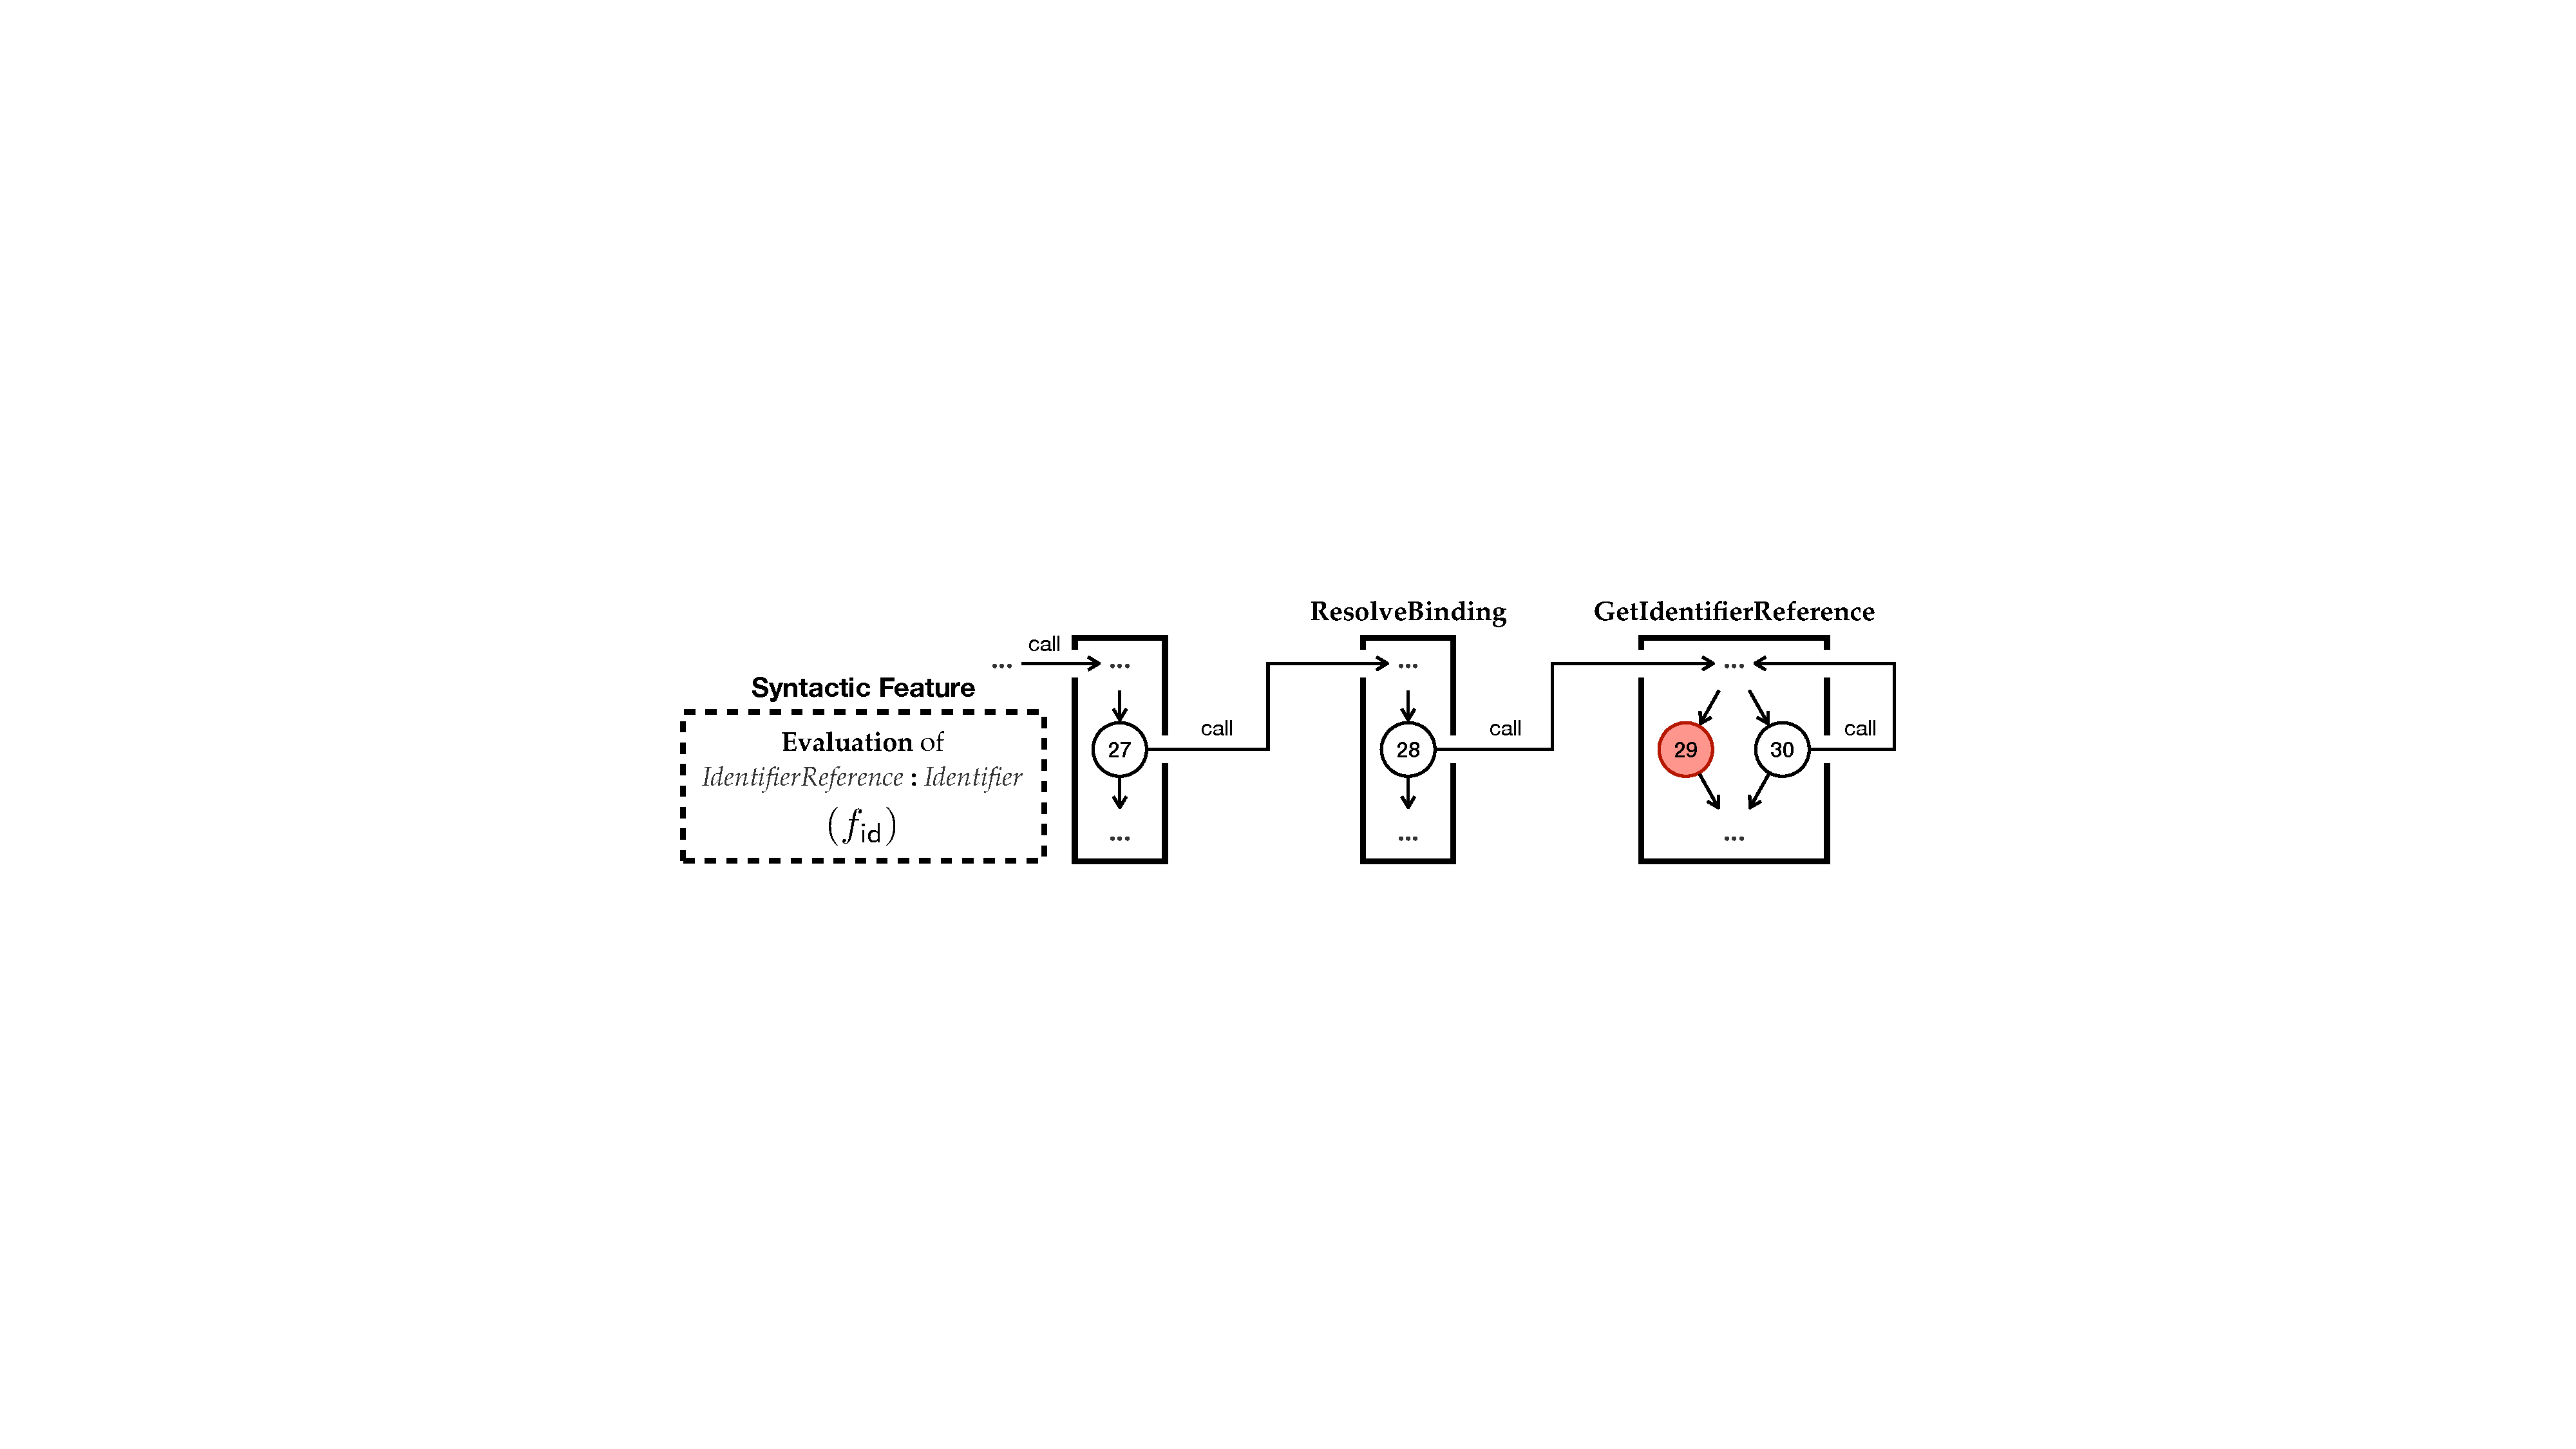
\includegraphics[width=0.85\textwidth]{img/spec-cfg-id}
  \caption{
    An excerpt from the CFG of abstract algorithms in ES13 related to $\idfeat$,
    a syntactic feature defined by the first alternative of
    \esnt{IdentifierReference} and its \textbf{Evaluation} SDO.
  }
  \label{fig:spec-cfg-id}
\end{figure}

We show two examples for FCPS node coverages in graph with graphs in
Figure~\ref{fig:spec-cfg} and Figure~\ref{fig:spec-cfg-id}.
%
First, consider the following two JavaScript programs as tests with the CFG in
Figure~\ref{fig:spec-cfg}:
%
\begin{equation}\label{equ:fcps-example1}
  \begin{array}{rcl}
    \test_0 \in \testset &=& \text{(a JavaScript program \jscode{2n + 1;})}\\
    \test_1 \in \testset &=& \text{(a JavaScript program \jscode{1 + 2n;})}\\
  \end{array}
\end{equation}
%
If we use FS node coverage, both tests $\test_0$ and $\test_1$ cover the same
FS-TR $(21, \addfeat)$, and one of them might be removed in the minimal test
set.
%
However, if we use FCPS node coverage, $\test_0$ and $\test_1$ cover different
FCPS-TRs $(21, (\addfeat, [1, 8, 12]))$ and $(21, (\addfeat, [1, 8, 14]))$,
respectively.
%
The other example is about the cycles in the call-site stacks with the graph in
Figure~\ref{fig:spec-cfg-id}.
%
It depicts an excerpt from the CFG of abstract algorithms in ES13 related to
$\idfeat$, a syntactic feature defined by the first alternative of
\esnt{IdentifierReference} and its \textbf{Evaluation} SDO. 
%
Assume that we do not remove cycles in the feature call paths $\fcpset$ during
the extraction algorithm $\extfcp$.
%
Then, since the algorithm \textbf{GetIdentifierReference} contains a
self-recursion, there exists an infinite number of possible feature call paths
from $\idfeat$ to node 29:
%
\begin{equation}\label{fcp-inf-example}
  (\idfeat, [27, 28]) \qquad
  (\idfeat, [27, 28, 30]) \qquad
  (\idfeat, [27, 28, 30, 30]) \qquad
  \cdots
\end{equation}
%
However, we remove cycles in feature call paths to resolve this issue, and there
exists only two possible feature call paths: $(\idfeat, [27, 28])$ and
$(\idfeat, [27, 28, 30])$.

%----------------------------------------%

Similar to the extension of FS coverages to $k$-FS coverages, we define a
$k$-FCPS coverage by extending the $\extfcp$ into $\extfcps{k}:
\css{\patset{\graph}} \rightarrow \fcpset^{\leq k}$ where $\fcpset^{\leq k} =
\featset^{\leq k} \times \css{\patset{\graph}}$:
%
\begin{equation}\label{equ:extfcps}
  \extfcps{k}([\node_1, \cdots, \node_m]) = \left\{
    \begin{array}{ll}
      (\epsilon, \epsilon) & \tif k = 0 \vee m = 0\\

      (\feats + \feat, [\node_m]) & \tif \featmap(\node_m) = \feat \wedge
      \extfcps{k-1}([\node_1, \cdots, \node_{m-1}]) = (\feats, \_)\\

      \fcps & \tif \fcps = (\epsilon, \epsilon)\\

      (\feats, [\node'_0, \cdots, \node'_i]) &
      \tif \fcp = (\feats, [\node'_0, \cdots, \node'_{m'}]) \wedge
      \exists i. \tst \node'_i = \node_m\\

      (\feats, \nodes + \node_m) & \tif \fcp = (\feats, \nodes)\\
    \end{array}
  \right.
\end{equation}
%
where $\fcps = \extfcps{k}([\node_1, \cdots, \node_{m-1}])$.

%----------------------------------------%

\begin{definition}[$k$-Limiting Feature Call Path-Sensitive ($k$-FCPS)
  Coverage]\label{def:k-fcps-cov}
  For a given graph coverage $\cov{\graph} = (\trset{\graph}, \cover)$, the
  \textit{$k$-limiting feature call path-sensitive ($k$-FCPS) coverage}
  $\kfcpcov{k}{\graph} = (\kfcptrset{k}{\graph}, \cover)$ is defined as follows:
  \begin{itemize}
    \item the set of \textbf{$k$-feature call path-sensitive test requirements
      ($k$-FCPS-TRs)} $\kfcptrset{k}{\graph}$ is a set of original TRs tagged
      with extends feature call paths bounded by $k$:
      \[
        \kfcptrset{k}{\graph} = \trset{\graph} \times \fcpset^{\leq k}
      \]
    \item a path $\pat$ \textbf{covers} a $k$-FCPS-TR $(\tr, \fcps)$ when $\pat$
      covers the original TR $\tr$ and $\fcps$ is the extended feature call path
      extracted from $\pat$:
      \[
        \pat \cover (\tr, \fcps) \iff \pat \cover \tr \wedge
        \extfcps{k}(\css{\pat}) = \fcps
      \]
  \end{itemize}
\end{definition}

%----------------------------------------%

\begin{figure}
  \centering
  \small
  \begin{tikzpicture}[every node/.style={draw=none}]
    \node (base)   at (0,1) {$\cov{\graph}=\kfcov{0}{\graph}=\kfcpcov{0}{\graph}$};
    \node (1-fs)   at (3,0) {$\fcov{\graph}=\kfcov{1}{\graph}$};
    \node (2-fs)   at (6,0) {$\kfcov{2}{\graph}$};
    \node (k-fs)   at (8,0) {$\cdots$};
    \node (1-fcps) at (3,2) {$\fcpcov{\graph}=\kfcpcov{1}{\graph}$};
    \node (2-fcps) at (6,2) {$\kfcpcov{2}{\graph}$};
    \node (k-fcps) at (8,2) {$\cdots$};
    \path[->]
    (1-fs) edge node[auto] {(1)} (base)
    (2-fs) edge node[auto] {(1)} (1-fs)
    (k-fs) edge node[auto] {(1)} (2-fs)
    (1-fcps) edge node[auto] {(2)} (base)
    (1-fcps) edge node[auto] {(3)} (1-fs)
    (2-fcps) edge node[auto] {(2)} (1-fcps)
    (2-fcps) edge node[auto] {(3)} (2-fs)
    (k-fcps) edge node[auto] {(2)} (2-fcps);
  \end{tikzpicture}
  \caption{
    The subsumption relations between $k$-FS and $k$-FCPS coverages.
  }
  \label{fig:subs}
\end{figure}

In addition, we prove Theorem~\ref{thm:subs} for the subsumption relations
between $k$-FS and $k$-FCPS coverages.
%
We first prove the Lemma~\ref{lem:subs} and prove the theorem using it.
%
Figure~\ref{fig:subs} depicts the subsumption relations between them using edges
annotated with the corresponding equation in Theorem~\ref{thm:subs}.

%----------------------------------------%

\begin{lemma}\label{lem:subs}
  Consider two graph coverages $\cov{\graph} = (\trset{\graph}, \cover)$ and
  $\cov{\graph}' = (\trset{\graph}', \cover')$.
  %
  If there exists a valid TR $\tr \in \trset{\graph}$ that satisfies the following
  condition for each valid TR $\tr' \in \trset{\graph}'$:
  %
  \begin{equation}\label{equ:subs-lemma}
    \forall \test \in \testset. \; \test \cover \tr \Rightarrow \test \cover' \tr'
  \end{equation}
  %
  Then, $\cov{\graph}$ subsumes $\cov{\graph}'$ ($\cov{\graph}
  \subs\cov{\graph}'$).
\end{lemma}
\begin{proof}
  Assume $T \sat \cov{\graph}$.
  %
  For a given valid TR $\tr' \in \trset{\graph}'$, let $\tr \in \trset{\graph}$
  be the valid TR satisfies (\ref{equ:subs-lemma}).
  %
  Then, there exists a test $\test \in T$ such that $\test \cover \tr$ because
  $\tr$ is valid and $T \sat \cov{\graph}$.
  %
  Finally, $\test \cover \tr'$ because of (\ref{equ:subs-lemma}).
\end{proof}

\begin{theorem}[Subsumption Relation]\label{thm:subs}
  For a given integer $k > 0$, the following three subsumption relations
  ($\subs$) between $k$-FS and $k$-FCPS coverages satisfy:
  \begin{enumerate}
    \item $\kfcov{k}{\graph} \subs \kfcov{(k-1)}{\graph}$
    \item $\kfcpcov{k}{\graph} \subs \kfcpcov{(k-1)}{\graph}$
    \item $\kfcpcov{k}{\graph} \subs \kfcov{k}{\graph}$
  \end{enumerate}
\end{theorem}

\begin{proof}
  We prove the first subsumption relation using Lemma~\ref{lem:subs}, but omit
  the other second and third ones because it is possible to prove them in a
  similar way.
  %
  Let $k > 0$.
  %
  For a given valid $(k-1)$-FS-TR $(\tr, \feats)$, there exists a test $\test
  \in \testset$ such that $\test \cover (\tr, \feats)$ because $(\tr, \feats)$
  is valid.
  %
  There exists a prefix path $\pat$ of $\patmap{\graph}(\test)$ such that $\pat
  \cover (\tr, \feats)$ ($\because$ (\ref{equ:test-cover}))
  %
  Then, a $k$-FS-TR $(\tr, \extfeats{k}(\css{\pat}))$ satisfies the condition
  (\ref{equ:subs-lemma}) because of the inductive definition of $\extfeats{k}$
  in (\ref{equ:extfeats}).
  %
  Hence, $k$-FS coverages subsumes $(k-1)$-FS coverages.
\end{proof}
